\section{Ziel}
\label{sec:Ziel}
Durch diesem Versuch werden die fundamentalen physikalischen Gesetze der Strahlenoptik untersucht. Dazu wird überprüft, ob sich monochromatisches Licht unter Beugung, Brechung 
und Reflexion der Theorie nach verhält.

\section{Theorie}
\label{sec:Theorie}
Licht ist eine elektromagnetische Welle. Daher kann Licht in komplexer Weise durch die Maxwell-Gleichungen beschrieben werden. Dies ist für die fundamentalen Gesetze der
Strahlenoptik nicht nötig. Es genügt Licht auf ein einfacheres Verhalten zu vereinfachen. Dazu wird Licht ,aufbauend auf den niederländischen Physiker 
\textit{Christiaan Huygens}, auf das Ausbreitungsverhalten reduziert. Gemäß des \textit{Huygensschen Prinzips} breitet sich Licht entlang der Wellennormalen aus. Die 
Wellennormale steht immer orthogonal zur \textit{Wellenfront} und ist in \autoref{fig:Huygensbrechung} durch einen roten Pfeil skizziert. Das Huygenssche Prinzip sagt nun aus,
dass sich die Welle ausbreitet, indem an jedem Punkt der Wellenfront eine neue radiale Elementarwelle gleicher Frequenz entsteht. Durch Überlagerung aller dieser Elementarwellen 
ergibt sich eine neue Wellenfront. Dies beschreibt eine gradlinige Propagation einer Lichtwelle ohne Veränderung des Ausbreitungsmediums. Trifft eine Welle mit diesem 
gedanklichem Modell nun auf ein unterschiedliches Medium wird die Welle \textit{gebrochen},\textit{gebeugt} und oder \textit{reflektiert}. Diese Wechselwirkung mit einem
anderem Medium entsteht, da sich Wellen, so auch die Elementarwellen nach Huygens, in unterschiedlichen Medien unterschiedlich schnell ausbreiten. Die drei genannten 
Wechselwirkungen treten dann in Abhänigkeit vom Licht und Beugungsmaterial auf. 

\begin{figure}
    \centering
    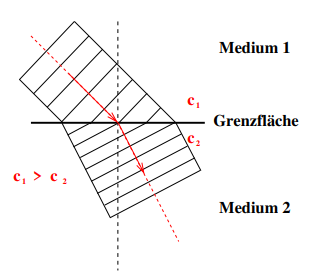
\includegraphics[width=0.5\textwidth]{content/HuygensscheBrechung.png}
    \caption{In dieser Abbildung ist schematisch das Huygenssche Prinzip dargestellt. \cite{v400}.}
    \label{fig:Huygensbrechung}
\end{figure}

\subsection{Reflexion}
\label{subsec:Reflexion}
Nun wird ein Lichtstrahl betrachtet, welcher in einem Winkelintervall von $[\qty{0}{\degree},\qty{90}{\degree}]$ zu Lot auf ein Grenzmedium trifft. Das Medium habe die 
Eigenschaft, dass das Licht nicht in es eintreten kann, sonder vollständig reflektiert wird. Diese Situation ist in \autoref{fig:Reflexion} dargestellt. In dieser Abbildung
beschreibt $\alpha_1$ den Einfallswinkel der Lichtwelle und $\alpha_2$ den \textit{Reflexionswinkel}. Für Reflexion gilt gemäß der Strahlenoptik 
\begin{equation}
  \label{eqn:Reflexionsgesetz}
  \alpha_1 = \alpha_2.
\end{equation}

\begin{figure}
  \centering
  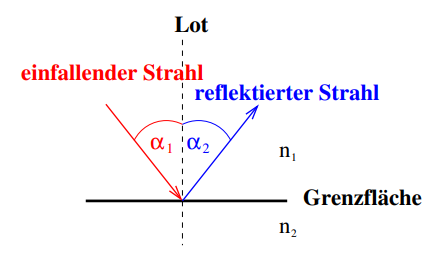
\includegraphics[width=0.5\textwidth]{content/Reflexion.png}
  \caption{In dieser Abbildung wird die Reflexion eines Lichtsstrahles gemäß der Strahlenoptik dargestellt. \cite{v400}.}
  \label{fig:Reflexion}
\end{figure}

\subsection{Brechung}
\label{subsec:Brechung}
Es wird dieselbe Ausgangslage betrachtet wie in \autoref{subsec:Reflexion}. Nun hat das Grenzmedium aber die Eigenschaft, dass das Licht vollständig in das Medium eindringen
kann. Aufgrund der unterschiedlichen Ausbreitungsgeschwindigkeiten läuft das Licht nun mit einem Brechungswinkel $\beta$ durch das Medium. Diese Situation wird in 
\autoref{fig:Brechung}dargestellt. Dieses Konzept kann ebenfalls aus dem 
Huygenschen Prinzip hergeleitet werden. Nach dem \textit{Snelliusschen Brechungsgesetz} verhalten sich Einfalls- und Brechungswinkel gemäß
\begin{equation}
  \label{eqn:Brechungsgesetz}
  n_1\sin\alpha = n_2\sin\beta
\end{equation}
zueinander.

\begin{figure}
  \centering
  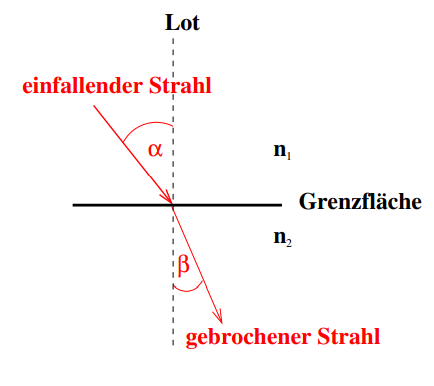
\includegraphics[width=0.5\textwidth]{content/Brechung.png}
  \caption{In dieser Abbildung wird die Brechung eines Lichtsstrahles gemäß der Strahlenoptik dargestellt. \cite{v400}.}
  \label{fig:Brechung}
\end{figure}

\subsection{Reflexion und Transmission}
\label{subsec:ReUTra}
In den letzten beiden Abschnitten wurde das auschließliche Auftreten eines bestimmten Effektes betrachtet. Allerdings tritt in der Regel meist eine Mischung aus beiden Effekten
auf. Das bedeutet ein Teil des Strahl wird reflektiert der andere Teil wird transmitiert und somit gebrochen. Die Gesetze der einzelnen Effekte ändern sich bei Überlagerung
nicht. Allerdings teilt sich die Intensität des einfallenden Strahles in reflektierte Intensität und transmitierte Intensität auf. Dabei beschreibt $R$ den Anteil der 
reflektierten Intensität an der einfallenden Intensität und $T$ den Anteil der transmitierten Intensität. Aufgrund der Energieerhaltung muss $R + T = 1$ gelten.

\subsection{Beugung}
\label{subsec:Beugung}
Die Beugung einer Welle kann nicht durch die Strahlenoptik beschrieben werden. Daher wird nun das Phänomen der Beugung durch \textit{Wellenoptik} beschrieben. Licht ist eine
elektromagnetische Welle, weshalb das Superpositionsprinzip gelten muss. Daher können zwei Lichtwellen miteinander interferieren. Beugung beschreibt allerdings das Phänomen,
dass eine Welle an einem Objekt gebeugt wird. Trifft eine Lichtwelle auf ein Objekt oder einen Spalt, welches oder welcher jeweils klein gegenüber der Wellenlänge sind tritt
nach der Wechselwirkung ein Interferenzmuster auf.   